\chapter{Estado da Arte}

Em seguida é demonstrado uma análise detalhada a respeito de tecnologias utilizadas para resolver problemas semelhantes, como também, este capítulo tem a finalidade de evidenciar os principais critérios utilizados para implementar a solução.

\section{Soluções Semelhantes}

Existem aplicativos no mercado com o intuito de atender o mesmo problema abordado neste trabalho, portanto esta seção possui o objetivo de abordar as principais funcionalidades de três das principais aplicações encontradas e selecionadas pelo fato de cada uma possuir mais de 1 milhão de usuários e com uma avaliação positiva dos usuários, recebendo notas acima de 4 em uma escala de 1 a 5.

\subsection{Moovit}

O Moovit \footnote{https://moovitapp.com/} possibilita que os seus usuários acompanhem todo o trajeto pelo aplicativo, a partir do momento em que você escolhe o destino, até a sua chegada. Com ele o usuário consegue encontre a melhor linha para chegar ao seu destino e recebe instruções sobre como chegar à estação ou parada mais próxima, do mesmo modo informa ao usuário quando está ele está chegando e em qual local descer. Como também, fornece programações atualizadas dos horários e atualizações de chegada em tempo real, recebidas do GPS dos ônibus e trens.

Com este aplicativo também é possível acompanhar em tempo real as informações atualizadas sobre atrasos e interrupções do serviço, engarrafamentos e novas obras, para lhe ajudar a navegar até o seu destino e, com isso, efetuar o planejamento de viagens por meio da visualização de rotas que lhe ajudam a chegar ao seu destino, através da comparação dos horários de partida, tempo total de caminhada até a sua estação, e rotas combinando diferentes meios de transporte.

Também é possível que os usuários reportem problemas encontrados em estações, linhas e horários, para informar os passageiros nas proximidades o que está acontecendo.

\begin{figure}[H]
\caption{Moovit - Tela de Visualização de Linhas}
\centering
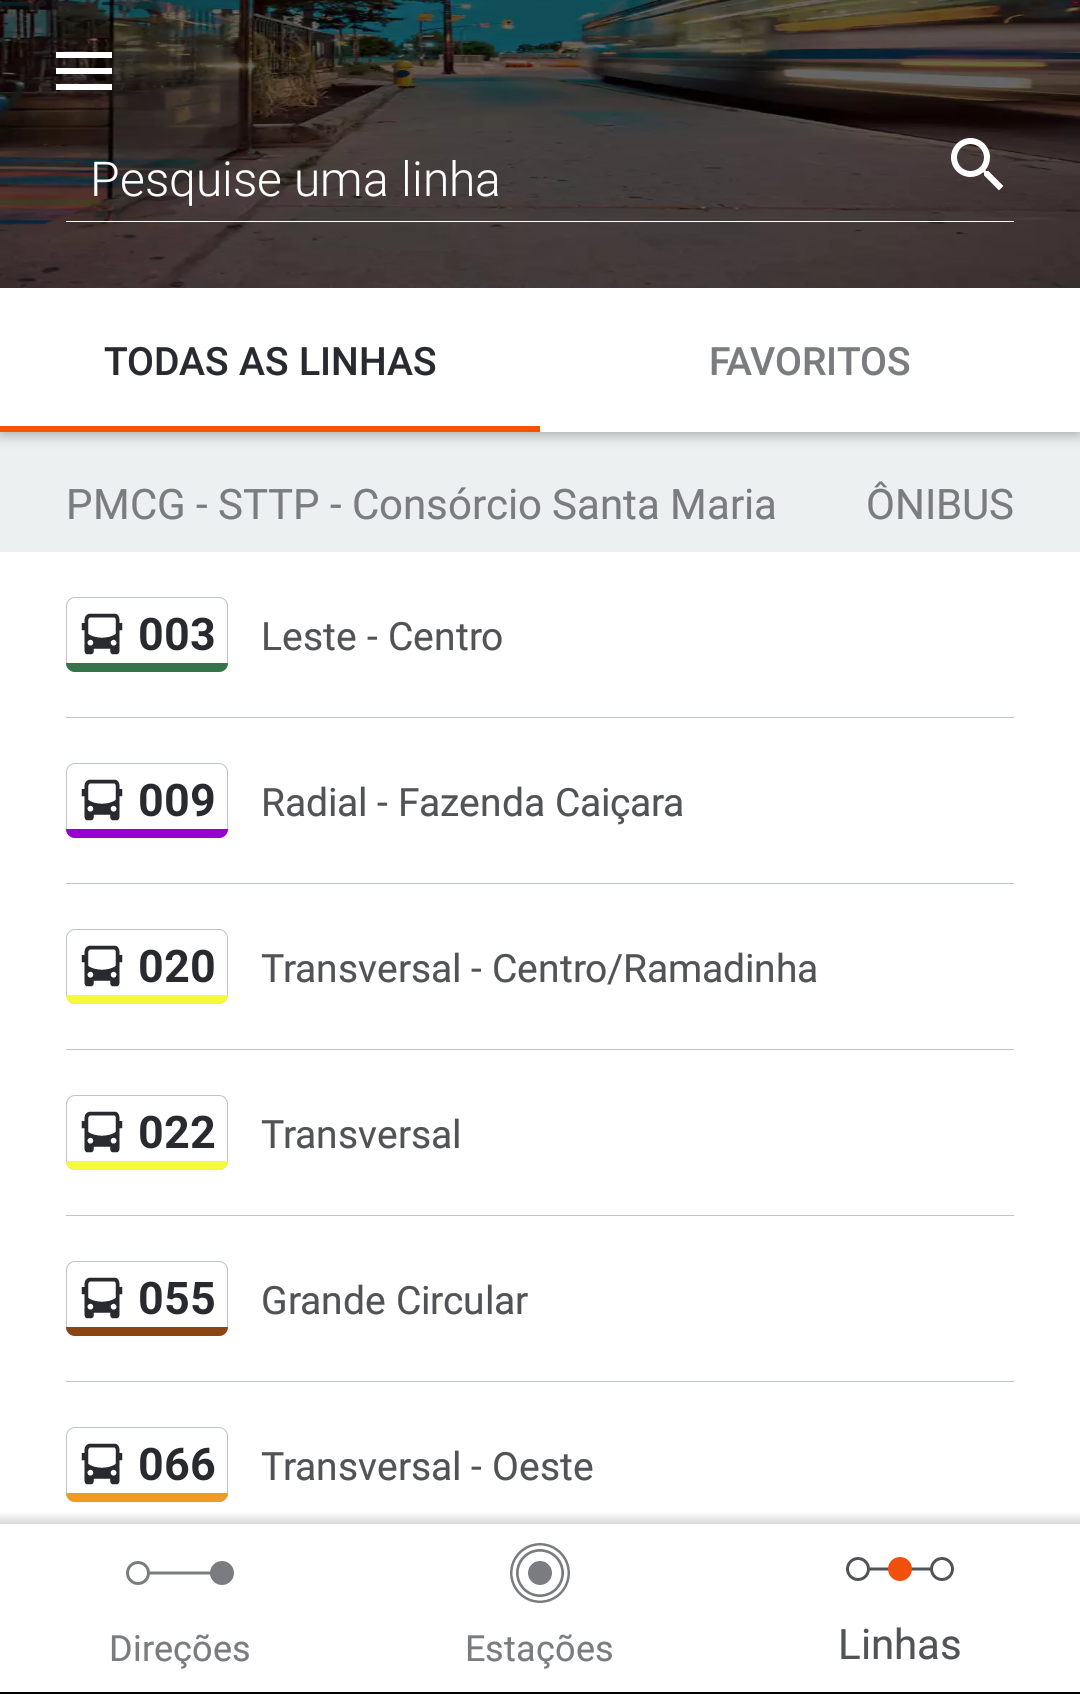
\includegraphics[width=.4\textwidth]{imagens/moovit.png}
\legend{Fonte: Autor}
\label{fig:moovit}
\end{figure}

\subsection{CittaMobi}

O CittaMobi \footnote{https://www.cittamobi.com.br/home/} é um aplicativo de acompanhamento dos transportes públicos que possibilita a previsão de tempo de chegada dos ônibus em tempo real, mostra a melhor rota de sua localização atual até o seu destino, vende bilhetes eletrônicos que funcionam como passagens para uso do ônibus, disponibiliza um botão para aviso de incidente grave e mostra o itinerários das linhas de ônibus.

Entre as funcionalidades do CittaMobi está a previsão de chegada dos ônibus que se da por meio da coleta da posição dos ônibus em tempo tempo real por meio de um GPS instalado no mesmo. Com o objetivo de garantir a precisão do horário de chegada em todas as paradas em seu percurso e, com isso, permite que os usuários percam menos tempo esperando. 

Com a utilização deste aplicativo é possível encontrar o melhor caminho até o seu destino, incluindo trechos a pé, de trem, ônibus ou metrô. Todas estas possibilidades são levadas em consideração ao traçar a melhor rota e demonstrar em um mapa detalhado o percurso definido.

O aplicativo ainda permite que os usuários gravem seus seus pontos favoritos para facilitar o uso do aplicativo, pois assim é possível facilitar a busca de informações sobre o ponto favorito, como por exemplo o horário de chegada dos ônibus e as linhas que passam por ele.

\begin{figure}[H]
\caption{CittaMobi - Tela de Busca de Rotas}
\centering
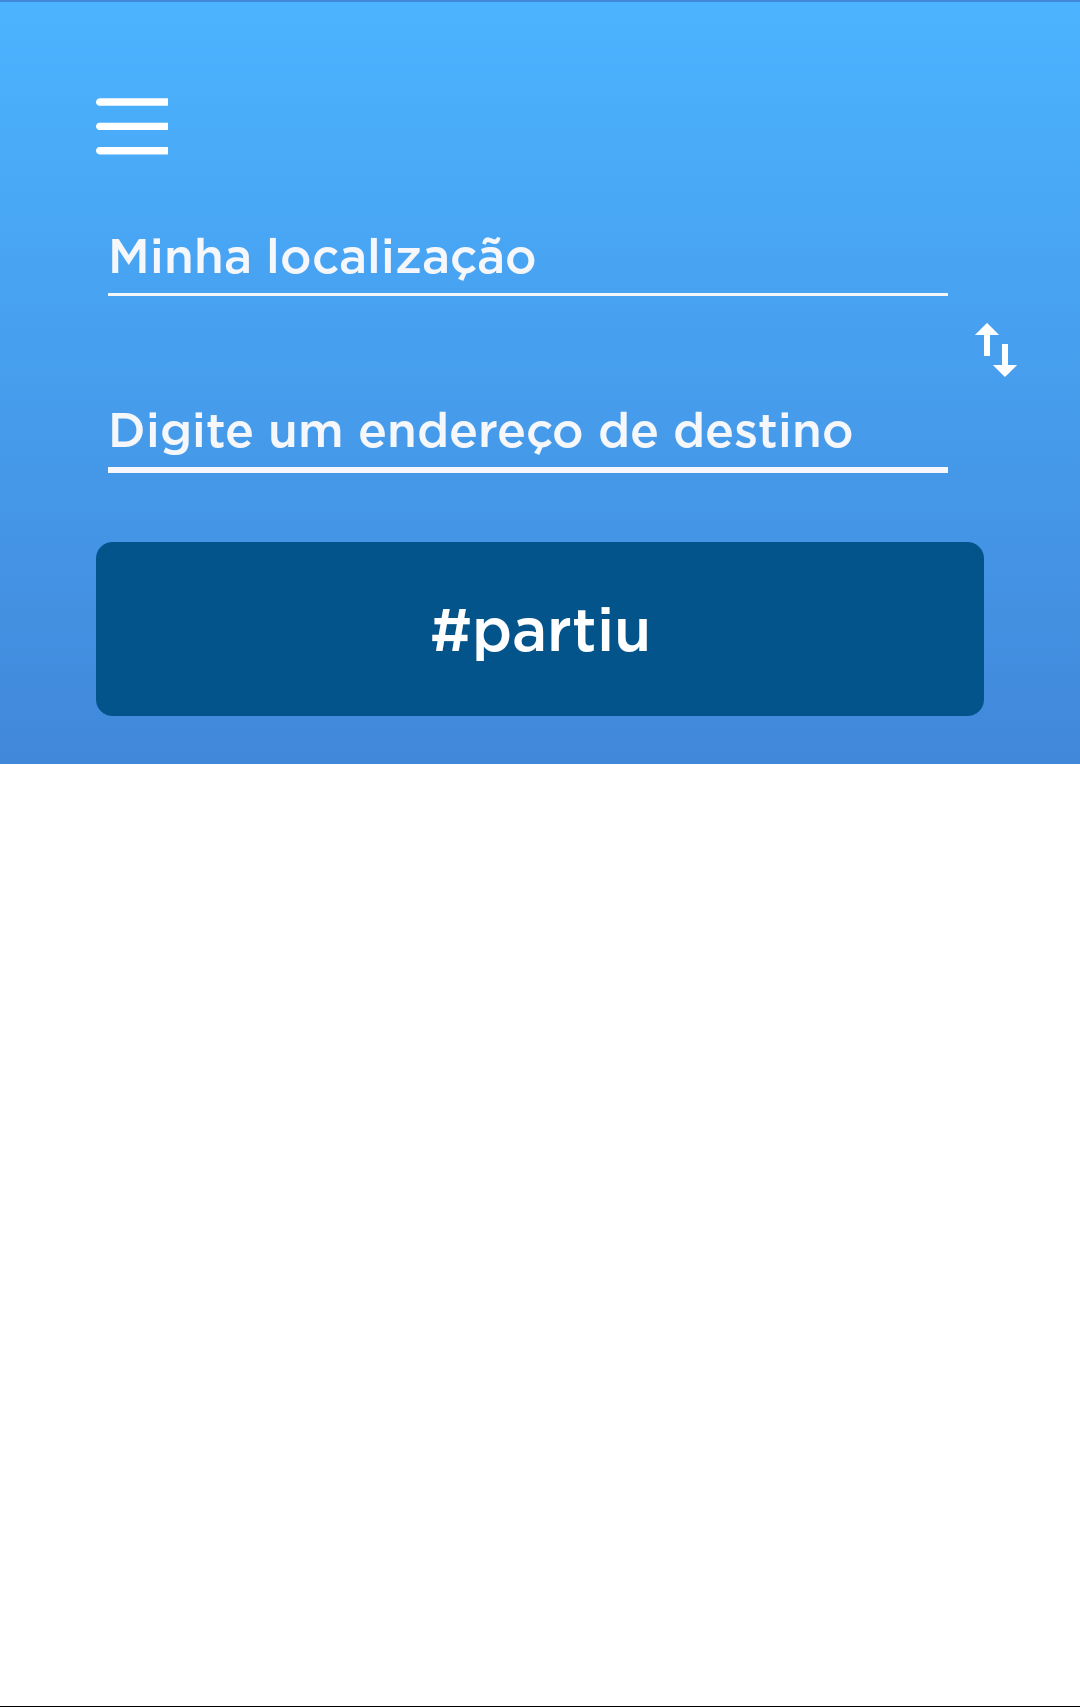
\includegraphics[width=.4\textwidth]{imagens/citta-mobi.png}
\legend{Fonte: Autor}
\label{fig:cittamobi}
\end{figure}

\subsection{Trafi}

O Trafi \footnote{https://www.trafi.com/} é um aplicativo de acompanhamento dos transportes públicos que possibilita o acompanhamento de sua cidade definida como favorita e a visualização dos detalhes em tempo real, todavia esta solução permanece funcional sem acesso a internet, limitando as suas funcionalidades, porém ainda é possível consultar informações importantes sobre as linhas, horários e exibir as rotas, em um mapa, das linhas disponíveis.

Com a utilização deste aplicativo é possível encontrar o melhor caminho até o seu destino, conectando todas as suas opções de transporte que incluem trechos de trem, ônibus, metrô, bicicletas públicas, carros compartilhados e motoristas de aplicativos. Ao conectar todos os transportes disponíveis o Trafi mostra ao usuário sua melhor opção pra chegada ao seu destino com base nos transportes disponíveis para a região solicitada, oferecendo a possibilidade do usuário comparar e escolher a melhor rota com base na eficiência, tempo ou custo.

O aplicativo ainda permite que os usuários gravem seus seus destinos favoritos para facilitar o uso do aplicativo, pois assim é possível facilitar a busca de rotas disponíveis para o seu destino favorito com base na sua localização atual e, com isso, o usuário não precisa digitar o mesmo endereço de destino repetidas vezes.


\begin{figure}[H]
\caption{Trafi - Tela de Detalhes da Linha Selecionada}
\centering
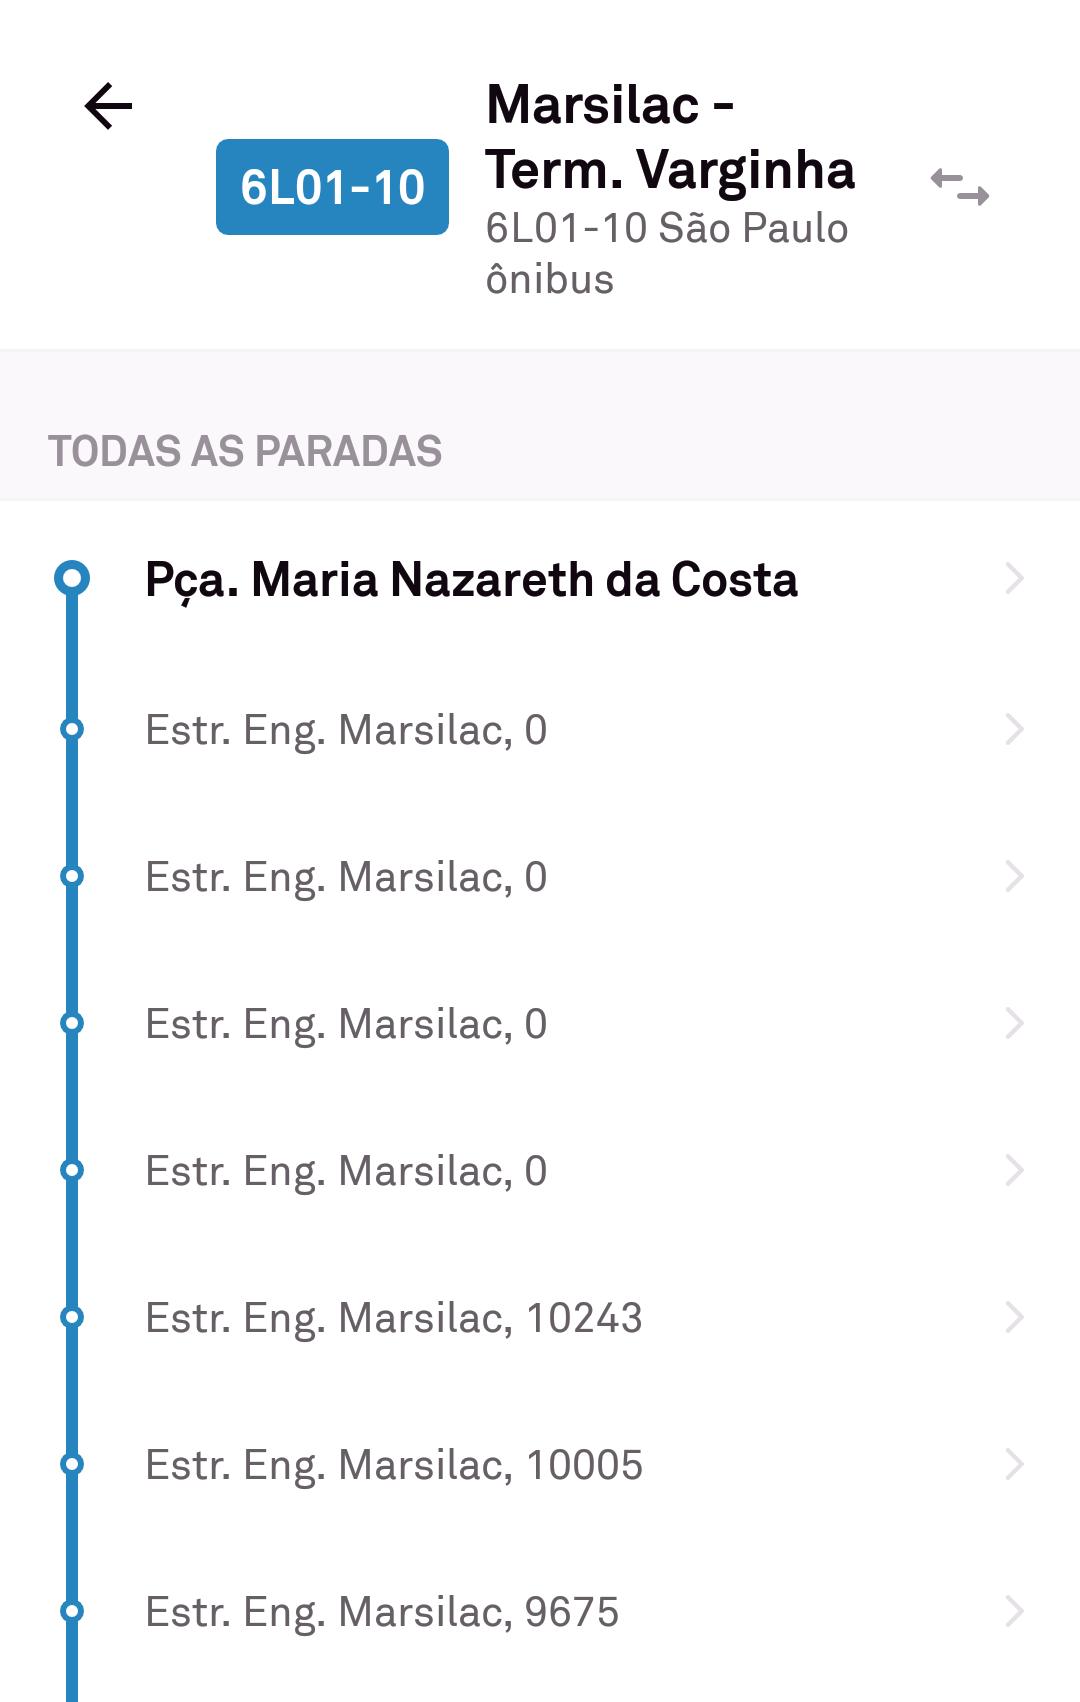
\includegraphics[width=.4\textwidth]{imagens/traffi.png}
\legend{Fonte: Autor}
\label{fig:trafi}
\end{figure}

\section{Análise das Soluções}

Ao analisar as soluções descritas neste capítulo, foram escolhidas algumas características que são essenciais para melhor atender a cidade de Picos. Todas as características escolhidas foram relacionadas as funcionalidades existentes em cada solução, As características selecionadas e a solução que as contempla podem ser vistas na Tabela \ref{tab:comparativo-solucoes}.

Ao analisar a Tabela \ref{tab:comparativo-solucoes}, é possível verificar que as soluções propostas neste capítulo abordam 5 das 7 características escolhidas, contudo nosso objetivo principal se deve a insatisfação do uso de transporte público na região de Picos e nenhuma das soluções encontradas atende essa necessidade e, ao analisar as aplicações existentes é evidente que não é de interesse destes aplicativos atender cidades menores, focando seus esforços em grandes centros urbanos, com múltiplos recursos e serviços que não se fazem necessários em cidades menores.

{\renewcommand{\arraystretch}{2}
\begin{table}[H]
\centering
\caption{Comparativo das Soluções Semelhantes}
\label{tab:comparativo-solucoes}
\begin{tabular}{ p{7cm} | c c c c }
\hline
\textbf{FUNCIONALIDADE} & \textbf{MOOVIT} & \textbf{CITTAMOBI} & \textbf{TRAFI} & \textbf{TOPIN} \\
\hline
Busca de Linhas & X & X & X & X \\ \hline
Visualiza os Horários das Linhas & X & X & X & X \\ \hline
Verifica Paradas Mais Próximas & X & X & X & X \\ \hline
Acompanha Transporte em Tempo Real & X & X & X & X \\ \hline
Busca de Linhas e Horários Offline & X & & X & X \\ \hline
Atende a Cidade de Picos &  &  &  & X \\ \hline
Ambiente Administrativo Para Empresa de Transporte &  &  &  & X \\ \hline
\end{tabular}
\legend{Fonte: Autor}
\end{table}

As características selecionadas para a comparação, foram determinadas como parâmetro para análise, com base em uma pesquisa efetuada com usuários do transporte público na região de Picos, que será melhor evidenciada no capítulo que se segue, portanto esses aplicativos podem ter mais funcionalidades que o Topin, todavia não possuem relação direta com o objetivo deste trabalho.